\documentclass[times, utf8, zavrsni]{fer}
\usepackage{booktabs, graphicx, listings, color, multirow, float}

\definecolor{dkgreen}{rgb}{0,0.6,0}
\definecolor{gray}{rgb}{1,1,1}
\definecolor{mauve}{rgb}{0.58,0,0.82}


\lstset{frame=tb,
  language=C++,
  aboveskip=3mm,
  belowskip=3mm,
  showstringspaces=false,
  columns=flexible,
  basicstyle={\small\ttfamily},
  numbers=left,
  numberstyle=\color[rgb]{0.205, 0.142, 0.73},
  keywordstyle=\color{blue},
  commentstyle=\color{dkgreen},
  stringstyle=\color{mauve},
  breaklines=true,
  breakatwhitespace=true,
  tabsize=3, 
  literate=%
  	{ć}{{\'c}}1
  	{č}{{\v{c}}}1
  	{š}{{\v{s}}}1
}

\begin{document}

% TODO: Navedite broj rada.
\thesisnumber{4334}

% TODO: Navedite naslov rada.
\title{Primjena genetskog programiranja na problem klasifikacije podataka}

% TODO: Navedite vaše ime i prezime.
\author{Ivan Vlašić}

\maketitle

% Ispis stranice s napomenom o umetanju izvornika rada. Uklonite naredbu \izvornik ako želite izbaciti tu stranicu.
\izvornik

% Dodavanje zahvale ili prazne stranice. Ako ne želite dodati zahvalu, naredbu ostavite radi prazne stranice.
\zahvala{Zahvaljujem se mentoru prof. dr. sc. Domagoju Jakoboviću na savjetima i pomoći pri izradi ovog završnog rada.

Također se zahvaljujem svojim roditeljima i obitelji na stalnoj podršci i razumijevanju tijekom školovanja.}

\tableofcontents

\chapter{Uvod}
Klasifikacija je problem razvrstavanja podataka u kategorije na osnovu skupine podataka za učenje čija je podjela već poznata. Kao primjer koji se u praksi često koristi, možemo navesti prepoznavanje spada li novi email pod neželjeni sadržaj ili ne. Razvojem računarske znanosti, a pogotovo strojnog učenja, došlo je do pojave različitih metoda rješavanja tog problema. Neke su bile više uspješne od drugih. Ovaj rad će pokušati pojasniti rješavanje problema klasifikacije podataka upotrebom genetskog programiranja koje se pokazalo kao dosta precizna metoda iako može dovesti do problema prevelike složenosti kod velike skupine podataka.

U početku ćemo se upoznati s problemom klasifikacije, njegovim najčešćim primjenama i prihvaćenim metodama rješavanja te osnovnim karakteristikama genetskog programiranja koje ga čine pogodnim za rješavanje ovog problema. Posebnu pažnju ćemo posvetiti algoritmima klasifikacije u obliku regresijskog modela i logičkih pravila. Pojasnit ćemo programski sustav implementiran uz ovaj rad, modele i operatore koje smo koristili kao i detaljne upute za korištenje. Analizirat ćemo rezultate dobivene primjenom navedenog sustava na testne primjere te donijeti zaključke o njegovoj optimiziranosti i kvaliteti dobivenih rješenja.

\chapter{Strojno učenje i problem klasifikacije}
U ovom poglavlju ćemo dati kratki pregled strojnog učenja i upoznati se s njegovim vrstama. Objasnit ćemo problem klasifikacije podataka i proučiti njegove najčešće primjene. Na kraju ćemo opisati neke od najznačajnijih algoritama koji se u današnje vrijeme koriste za rješavanje tog problema kao i njihovu uspješnost.

\section{Strojno učenje}
Strojno učenje je grana računarske znanosti koja se razvila iz prepoznavanja uzoraka i teorije učenja u umjetnoj inteligenciji. Podrazumijeva programiranje računala tako da optimiziraju neki kriterij uspješnosti temeljem podatkovnih primjera ili prethodnog iskustva. Strojno učenje je veliki razvoj doživjelo osamdesetih godina prošlog stoljeća kad se počelo udaljavati od umjetne inteligencije i razvijati kao zasebna grana računarske znanosti.

Strojno učenje možemo podijeliti na nadzirano, nenadzirano i podržano učenje. Nadzirano učenje se koristi ulaznim skupom podataka kako bi učilo i izgradilo model predviđanja. Podaci za učenje se sastoje od primjera koji imaju vektor ulaznih podataka i predviđen izlaz. Algoritmima nadziranog učenja se ti podaci analiziraju i stvara se funkcija koja se može koristiti za mapiranje novih primjera. Ovim postupcima mogu se rješavati dvije vrste problema: klasifikacija i regresija. Kod klasifikacije primjeru pridružujemo klasu kojoj taj primjer pripada, dok kod regresije primjeru pridružujemo neku kontinuiranu vrijednost.

Za razliku od nadziranog učenja, nenadzirano učenje ne koristi podatke za učenje. Kod ove vrste učenja dani su nam podaci bez ciljne vrijednosti i naš je zadatak pronaći pravilnosti među njima. Tipično se koristi kod eksplorativne dubinske analize podataka, u biologiji za grupiranje organizama prema njihovim značajkama, grupiranju sličnih dokumenata, grupiranju DNA-mikropolja i slično. Koriste se grupiranje, procjena gustoće i smanjenje dimenzionalnosti.

Podržano učenje je učenje strategije na temelju serije izlaza. Tipično se koristi kod igara, robotike i upravljanja te višeagentnih sustavima. Pristup temelji na agentima koji ovisno o kvaliteti postignutih rezultata postižu nagrade. Cilj svakog agenta je maksimizirati dobivenu nagradu i time temelji uspjeh svojih strategija. 

\section{Klasifikacija podataka}

Kao što je već objašnjeno u uvodu poglavlja, problemi klasifikacije podataka se rješavaju postupcima nadziranog učenja. Svakom primjeru pridružujemo određenu klasu, odnosno razred kojoj pripada. Primjer možemo definirati kao vektor značajki gdje \textit{n} predstavlja dimenziju vektora, $X = (x_1, x_2,..., x_n)^T$. Vektor predstavlja ulazni prostor (engl. \textit{input space}) ili prostor primjera (engl. \textit{instance space}). Kod nadziranog učenja unaprijed nam je poznata klasa kojoj pripada primjer iz skupa učenja. Cilj klasifikacije je određivanje nepoznatih klasa ili grupa u podacima, to jest svrstati nove, već neviđene podatke u neki od već unaprijed poznatih klasa. Najjednostavniji je slučaj u kojem se podaci moraju svrstati u samo jedan razred. Kod više razreda, radi se o klasifikaciji s višestrukim oznakama. Ako se ograničimo samo na dvije klase, klasifikator nazivamo binarni klasifikator. 

Skup primjera za učenje sastoji se od parova primjera i pripadnih oznaka. Možemo ga prikazati tablično kao:

\begin{center}
 \begin{tabular}{||c c c c||} 
 \hline
 $x_1$ & $x_2$ & ... & y  \\ [0.5ex] 
 \hline\hline
 $x_1^{(1)}$ & $x_2^{(1)}$ & ... & $y^{(1)}$ \\ 
 \hline
 $x_1^{(2)}$ & $x_2^{(2)}$ & ... & $y^{(1)}$ \\
 \hline
 \vdots & \vdots &  & \vdots \\
 \hline
 $x_N^{(1)}$ & $x_N^{(1)}$ & ... & $y^{(N)}$ \\ [1ex] 
 \hline
\end{tabular}
\end{center} 


gdje je N ukupan broj primjera, a \textit{i} indeks primjera. Skup ulaznih oznaka označavamo s $(x^{(i)})_{i=1}^N$, a izlaznih s \textit{y}. Zadaća klasifikacijskog algoritma jest naučiti hipotezu koja određuje pripada li neki primjer određenoj klasi ili ne. Da bi u tome uspio, potrebno je izgraditi klasifikator. Ako klasifikator dobro generalizira ispravno će klasificirati još neviđene podatke. Važno je napomenuti da uspjeh klasifikatora u velikoj mjeri ovisi o svojstvima podataka koje je potrebno klasificirati. Ne postoji klasifikator koji radi najbolje za sve probleme (pojava koja je poznatija pod imenom \textit{no free lunch theorem}). Određivanje primjerenog klasifikatora za neki problem je dosta složen i težak problem koji nije uvijek moguće riješiti. Učenje hipoteze je loše definiran problem (engl. \text1it{ill-posed problem}). Primjeri za učenje nisu sami po sebi dovoljni da bi se hipoteza jednoznačno definirala. Svojstvo hipoteze da odredi klase još neviđenih primjera naziva se generalizacija. 

Jedan od glavnih problema do kojih može doći je problem šuma. Šum je neželjena anomalija u podacima koja je uzrokovana različitim uzrocima poput nepreciznosti pri mjerenju značajki, pogreški u označavanju, nejasnih granica klasa i postojanju skrivenih značajki. U načelu, šum nije moguće razdvojiti od pravih podataka. Danas klasifikacija ima mnoge primjene. Koristi se u računalnom vidu, prepoznavanju govora, klasifikaciji dokumenata i slično. Svi ovi i mnogi drugi problemi se rješavaju različitim algoritmima od kojih svi imaju svoje pozitivne i negativne strane, kao i različite uspješnosti. U sljedećem poglavlju ćemo razmotriti neke od najčešćih algoritama koji se koriste u praksi kao i njihove značajke. 

\section{Najznačajniji algoritmi za rješavanje problema klasifikacije}
Algoritama za rješavanje problema klasifikacije postoji mnogo. Razlikuju se po svojoj jednostavnosti primjene, točnosti i razumljivosti. Uspješnost algoritama u velikoj mjeri ovisi o problemu kojeg rješavamo. Ponekad nam je važnija brzina klasifikatora od njegove točnosti, a u drugim slučajevima je važnije da klasifikator ima veliku točnost nego brzinu ili jednostavnost. Među algoritme linearne klasifikacije spadaju Fisherova linearna diskriminanta i Naivni Bayes klasifikatori koji su se u početku pokazali dosta učinkovitima za rješavanje složenih problema, no detaljna analiza 2006. godine je pokazala da postoje drugi algoritmi koji su dosta bolji, poput algoritma \textit{random forest}. U tu skupinu još spadaju logistička regresija i \textit{perceptron}. Jedan od češće korištenih algoritama je i metoda potpornih vektora (engl. \textit{Support Vector Machine}) koji se bazira na učenju razdvajanjem funkcija i estimacije funkcije u regresiji. U velikoj upotrebi su i neuronske mreže koje su u širom smislu replika ljudskog mozga kojom se nastoji simulirati postupak učenja. To je skup međusobno povezanih jednostavnih procesnih elemenata koji se nazivaju čvorovi ili neuroni, i čija se funkcionalnost zasniva na biološkom neuronu. Neuronske mreže su vrlo dobre u procjeni nelinearnih odnosa uzoraka, mogu raditi s nejasnim ili manjkavim podacima, mogu raditi s velikim brojem varijabli i prilagođavati se okolini što ih čini pogodnim za probleme klasifikacije. Još neki od poznatijih metoda i algoritama su kvadratna metoda koja je dizajnirana za situacije kada karakteristike svake grupe imaju normalnu distribuciju te metoda kernel procjene.

Za probleme klasifikacije također se može koristiti i genetsko programiranje koje se zasniva na razvoju stabala odluke. Prednost genetskog programiranja leži u činjenici da može otkriti manje vidljive veze između podataka. Više o tome će biti objašnjeno u sljedećih nekoliko poglavlja.


\chapter{Genetsko programiranje}
U ovom poglavlju ćemo se detaljnije upoznati s genetskim programiranjem i vrstama koje se danas koriste. Objasnit ćemo probleme za čije je rješavanje pogodno genetsko programiranje kao i načini do kojih algoritmi dolaze do rješenja.

Genetsko programiranje je optimizacijska tehnika koja spada pod skupinu evolucijskih algoritama. Radi na principu simulacije evolucije, bolja rješenja preživljavaju i svoja svojstva prenose u sljedeće generacije dok loša izumiru. Kao i u prirodi, koriste se mehanizmi selekcije, križanja i mutacije čime možemo doći do raznolikog broja jedinki i uspješno se približiti dovoljno dobrom rješenju promatranog problema. Razvoj genetskog programiranja možemo pratiti od pedesetih godina prošlog stoljeća, no tek šezdesetih i sedamdesetih godina su postali šire prepoznati kao pogodna tehnika za rješavanje optimizacijskih problema. Većem napretku je pridonio John R. Koza koji je GP primijenio na velikom broju optimizacijskih problema i problema pretraživanja različite složenosti. Devedesetih se genetsko programiranje uglavnom koristilo za relativno jednostavne probleme budući da su izračuni dosta računalno intenzivni čemu računala tog doba nisu bila dorasla. U zadnjim godinama, zbog velikog napretka u razvoju procesora, genetsko programiranje se koristi za sve širi spektar problema poput sortiranja, pretraživanja, elektroničkog dizajna i mnogih drugih. 

Genetsko programiranje se često uspoređuje sa genetskim algoritmima. Međutim, postoje određene razlike. Kod genetskog programiranja rješenje je prikazano računalnim programom. Rješenje je onaj program koji daje rješenje zadanog problema u u najkraćem roku. Kod genetskih algoritama postoje različite reprezentacije rješenja ovisno o problemu koji rješavamo. Rješenje se može predstavljati brojkom, nizom bitova ili brojeva i drugima. Još jedna od većih razlika je duljina rješenja. Kod genetskog algoritma duljina rješenja se kroz evaluaciju ne mijenja, dok kod GP-a stabla često mijenjaju dubinu, veličinu i širinu. To često dovodi do problema prekomjernog rasta zbog čega je potrebno implementirati određena ograničenja duljine rješenja, poput dubine stabla ili broja čvorova.

U sljedećim potpoglavljima ćemo se detaljnije upoznati o načinu na koji genetsko programiranje radi.

\section{Stvaranje početne populacije}
Algoritam započinje nultom generacijom koja se stvara na temelju slučajnog odabira. Ova generacija nema nikakva optimizacijska svojstva, služi samo kao temelj za stvaranje i razvoj boljih jedinki u sljedećim generacijama. Postoje različiti načini kojima gradimo početnu generaciju, no najčešće korištene metode su \textit{Full} i \textit{Grow}.

\subsection{Metoda full}
Stvaranje stabala kod \textit{Full} metode započinje slučajno izabranom funkcijom koja predstavlja korijen. Potom rekurzivno stvaramo sljedeće razine stabla dok ne dođemo do maksimalno predviđene dubine. Tijekom ovog procesa čvorove biramo samo iz skupa operatora. Na posljednjoj razini odabiremo čvorove isključivo iz skupa završnih znakova.

\subsection{Metoda grow}
Ova metoda je slična prijašnjoj s razlikom da u svakom trenutku stvaranja čvorove možemo birati i iz skupa završnih znakova. Gradnjom stabala na ovaj način nećemo uvijek doći do maksimalne dubine zbog čega su stabla izgrađena ovom metodom dosta raznolikija i manje složena.

\subsection{Metoda ramped half-and-half}
Najčešća metoda korištena za stvaranje nulte populacije je metoda \textit{ramped half-and-half}. Polovica jedinki se stvara \textit{full} metodom, a druga polovica \textit{grow}. Određena je samo maksimalna dubina stabala, a jedinke se stvaraju za svaku dubinu, sve do maksimalne. 

Prednost ove metode je što stvara jedinke s dobrom raspodjelom po veličini i strukturi.
\section{Procjena dobrote jedinke}
Procjena dobrote jedinke uvelike ovisi o problemu kojim se bavimo. Predstavljena je funkcijom dobrote \engl{fitness function}. Ovisno o veličinama koje dobijemo primjenom funkcije dobrote možemo utvrditi kvalitetu pojedinog rješenja. Pravilno implementirana funkcija dobrote je važna jer o njoj u velikoj mjeri ovisi koja će rješenja ostati u razmatranju, a koja ne. Dobrotu neke jedinke možemo definirati kao mjeru kvalitete tog rješenja u zadanom prostoru rješenja. Primjerice, kod traženja maksimuma neke funkcije, dobrotu možemo prikazati kao vrijednost koju ta funkcija ima za pojedinu jedinku. Kod problema stvaranja rasporeda, dobrotu možemo procijeniti kao postotak predavanja koja se ne poklapaju, vremenskom intervalu koji studenti imaju između uzastopnih predavanja i slično. 

Definiranje funkcije dobrote je jedan od ključnih problema genetskog programiranja jer je potrebno da bude što preciznija, a što jednostavnija budući da je njeno evaluiranje potrebno obavljati u svakoj generaciji na cjelokupnom skupu jedinki. 

\section{Genetski operatori}

\subsection{Selekcija}
Jedan od centralnih mehanizama genetskog programiranja je selekcija. Ona omogućava boljim jedinkama da prenesu svoje "gene" u sljedeće generacije algoritma. Dobrota jedinke se zasniva na funkciji dobrote koju smo već opisali. Operatori selekcije i njihov utjecaj se mogu okarakterizirati kroz nekoliko parametara:

\begin{itemize}
\item{vrijeme preuzimanja,}
\item{selekcijski intenzitet,}
\item{momenti razdiobe dobrote}
\end{itemize}

Vrijeme preuzimanja je vrijeme potrebno operatoru selekcije da generira populaciju u kojoj se nalazi samo najbolje rješenje. To je vrijeme od prve generacije pa do nastanka generacije koja je popunjena samo jedinkama najboljeg rješenja ako koristimo samo mehanizam selekcije. Ako je mehanizam selekcije pravilan, u svakoj generaciji bi trebali imati sve bolja rješenja.

Selekcijski intenzitet je povećanje srednje dobrote populacije prije i poslije primjene operatora selekcije, podijeljenog sa standardnom devijacijom populacije:

\[ I = \frac{\bar{f_s} - \bar{f}}{\sigma} \]

$\bar{f} $ predstavlja prosječnu dobrotu rješenja u populaciji roditelja,  $\bar{f_s} $ predstavlja prosječnu dobrotu rješenja u populaciji djece, dok je $\sigma$ standardno odstupanje u populaciji roditelja.

\textit{r}-ti centralni moment razdiobe dobrote populacije rješenja veličine $n$ se računa prema izrazu:

\[ \mu_r = \frac1{n}\sum_{i=1}^{n}(f_i - \bar{f})^r \]

gdje je $f_i$ dobrota rješenja, a $\bar{f}$ srednja vrijednost dobrote za čitavu populaciju. 

U nastavku ćemo se upoznati s nekim od često korištenih vrsta selekcije.

\subsubsection{Proporcionalna selekcija}

Proporcionalnu selekciju možemo slikovito prikazati kao kotač ruleta gdje je svakom rješenju u populaciji pridružen isječak čija je površina proporcionalna dobroti rješenja. Tako najbolja jedinka ima najveći isječak kotača i najveću šansu za odabirom, dok će kod onih manje dobrih biti obrnuto.

\subsubsection{Turnirska selekcija}

Kod turnirske selekcije iz populacije izvlačimo slučajni uzorak od \textit{s} rješenja te odabiremo ono rješenje iz tog uzorka koje ima najveću dobrotu. 

Turnirska selekcija koja u populaciji od \textit{n} jedinki izvlači uzorak od njih \textit{s} naziva se \textit{s}-turnirska selekcija.

\subsection{Križanje}
Križanje je analogno biološkoj spolnoj reprodukciji. Križanjem dolazi do rekombiniranja genetskog materijala dvaju roditelja. Rezultat su dvije jedinke djece koje od svakog roditelja nasljeđuju dio genetskog materijala i koje će vjerojatno imati bolju dobrotu. U slučaju da se to ne dogodi loša rješenja će brzo "odumrijeti" mehanizmima selekcije koji će ih rjeđe birati za prijenos u sljedeće generacije. Ovisno o načinu prikaza jedinke postoje različite vrste križanja koje između ostaloga uključuju uniformno križanje koje se koristi kod jedinki predstavljenih kao niz bitova, aritmetičko, diskretno linearno križanje i drugi. Na slici 3.1 se nalazi primjer križanja na kojem se primjećuje kako nastala djeca nasljeđuju genetski materijal svojih roditelja.

\begin{figure}[htb]
\centering
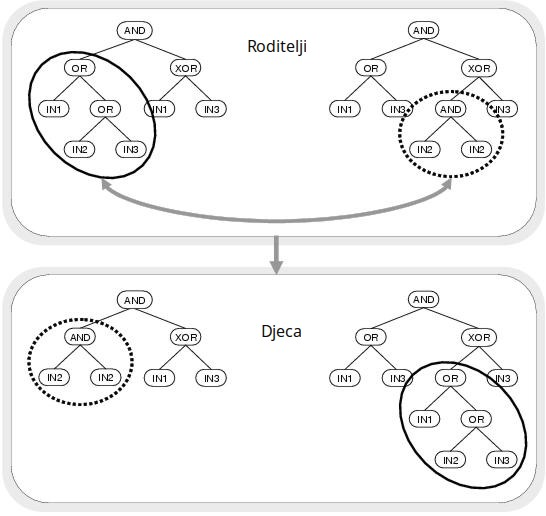
\includegraphics[scale=0.6]{images/krizanje}
\caption{Primjer križanja}
\end{figure}

\subsection{Mutacija}
Mutacija omogućava genetsku raznolikost jedinki čime se mogu dobiti bolja ili lošija rješenja. U generaciji se bira udio jedinki koji će sudjelovati u mutaciji ili vjerojatnost odabira mutacije za svaku pojedinu jedinku. Kod jedinki prikazanih stablima mutacija se obavlja tako da se nasumično odabere čvor koji se briše zajedno sa svojim podstablima. Na njegovom mjestu se generira novo podstablo stvoreno slučajnim odabirom. Pri tome je potrebno paziti da ne dođe do prekoračenja postavljenih ograničenja poput dubine stabla ili broja čvorova. Na slici 3.2 je prikazan primjer mutacija jedinke predstavljene stablom. 


\begin{figure}[htb]
\centering
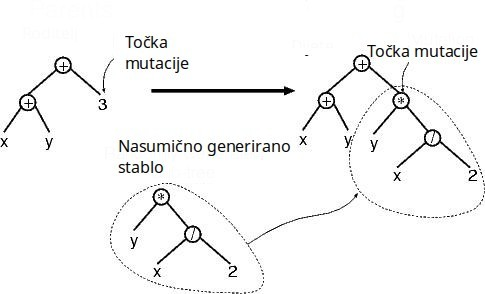
\includegraphics[scale=0.6]{images/mutacija}
\caption{Mutacija jedinke predstavljene stablom}
\end{figure}

\section{Problemi genetskog programiranja}
Kao što smo već napomenuli, kod genetskog programiranja možemo naići i na određene probleme. To je prije svega problem prebrzog rasta jedinki (engl. \textit {bloat}). Ako je jedinka prikazana u obliku stabla, problem se očituje kao nekontrolirani rast veličine stabla, to jest broja čvorova i dubine bez poboljšanja dobrote. To može dovesti do dugog trajanja evaluacije većih jedinki i nerazumljivosti i nečitljivosti rješenja. Predloženi su različiti mehanizmi rješavanja tog problema koji između ostalog uključuju kažnjavanje prevelikih jedinki, odbacivanje onih jedinki koji prelaze dopuštena ograničenja te njihova zamjena novim ili podrezivanje stabala (engl. \textit{tree pruning}). 

\section{Primjena genetskog programiranja na problem klasifikacije}
U ovom potpoglavlju ćemo se detaljnije upoznati s načinom na koji se genetsko programiranje koristi za rješavanje problema klasifikacije podataka. Klasifikacija je raširen problem s kojim se i nesvjesno suočavamo svaki dan. Na primjer, prepoznavanje lice pojedinaca koje smo prije upoznali, vrsta životinja, biljaka i hrane i drugih objekata iz okoline. Koristi se i u složenim znanstvenim domenama poput medicine gdje može pomoći u dijagnozi pacijenata na osnovu povijesti bolesti drugih pacijenata sa sličnim simptomima. 

S obzirom na raširenost ovog problema važno je razviti računalne mehanizme sposobne rješavanja problema klasifikacije u slučajevima kada je to za ljude presloženo i vremenski zahtjevno. Generalni oblik klasificiranja podrazumijeva prepoznavanje klasa kojima određeni primjerci problema pripadaju na osnovu atributa ili svojstava ispitnih primjeraka. Na osnovu ispitnih primjeraka možemo razviti model koji će predviđati klasu kojoj pripadaju novi, još nesvrstani primjerci.

Kroz povijest razvoja klasifikacije koristili su se različiti algoritmi i načini rješavanja tog problema. Genetsko programiranje je relativno novo i brzo razvijajuće područje koje se u široj primjeni našlo tek u zadnjih nekoliko desetljeća.

Model na kojem ćemo se zadržati u ovom radu je reprezentacija regresijskim stablima koje koristimo za klasifikaciju numeričkim izrazima. U kombinaciji s aritmetičkim operacijama koristit ćemo se i logičke izraze poput \textit{if-then-else} operacija koje se često koriste u računalnim programima. Ovakav način prikaza rješenja se pokazao relativno uspješnim u praktičnim primjenama poput klasifikacije rukopisa, bolesti, prepoznavanja objekata i slično. 

Primjer stabla i pripadajuće funkcije koja ovisi o ulaznim parametrima X i Y prikazan je na slici 3.3

\begin{figure}[htb]
\centering
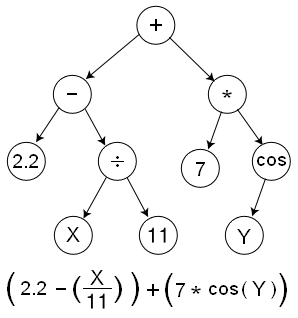
\includegraphics[scale=0.6]{images/stablo}
\caption{Stablo odluke}
\end{figure}

Klasifikator numeričkih izraza se definira kao bilo koja funkcija koja vraća numeričku vrijednost. Funkcija se sastoji od matematičkih operacija, uključujući aritmetičke operacije i druge poput sinusa, kosinusa ili logaritma. Kao što smo prije napomenuli, funkcije mogu sadržavati i operatore usporedbe kao ako-onda-ili izraz. Klasifikator numeričkih izraza provodi klasifikaciju pomoću varijabli koje su mu predane kao ulaz i na izlazu daje numeričku vrijednost. Ta numerička vrijednost se onda mora interpretirati u jednu od mogućih klasa za zadani problem.   

Važnost će biti na preciznosti modela koji nastaju genetskim programiranjem. Iako postoje drugi faktori o kojima može ovisiti kvaliteta promatranog rješenja poput veličine programa, razumljivosti, vremenskoj izvedbi i slično, njih ćemo svrstati u drugi plan. Na osnovu toga, kvalitetna rješenja će biti ona koja imaju najveći preciznost izvođenja klasifikacije, bez obzira na ostale promatrane uvjete.

Cilj je za zadane primjere proizvesti program koji će što preciznije klasificirati primjere i u velikom postotku predviđati pripadnost primjeraka problema zadanim klasama. 

\chapter{Programsko ostvarenje}

U ovom poglavlju ćemo detaljnije opisati programsko ostvarenje i opisati na koji smo način rješavali problem klasifikacije podataka upotrebom genetskog programiranja. Upoznati ćemo se s radnim okruženjem ECF-a, opisati genetske operatore koje smo koristili i objasniti prikaz dobivenog rješenja.

\section{Radno okruženje ECF}

ECF \engl{Evolutionary Computation Framework} je radno okruženje za rješavanje problema evolucijskog računanja koje se razvija na Fakultetu elektrotehnike i računarstva u Zagrebu pod vodstvom izv. prof. dr. sc. Domagoja Jakobovića. Napisano je u programskom jeziku C++. 

Za korištenje ECF-a možemo kombinirati i parametrizirati sljedeće komponente:

\begin{itemize}
\item Genotype
\item Algorithm
\item Evolutionary system
\end{itemize}

\textbf{Genotype} je osnovna komponenta ECF-a. Svaka jedinka u populaciji ima jednog ili više genotipa koje je najjednostavnije definirati u konfiguracijskoj datoteci. Genotip je jedina komponenta koju je potrebno definirati, sve ostale mogu koristiti pretpostavljene vrijednosti. Svaki genotip ima svoju strukturu i genetske operatore križanja i mutacije. U ovom radu ćemo koristiti izvedeni razred \textbf{Tree} koji predstavlja stablasti kromosom genetskog programiranja.

\textbf{Algorithm} predstavlja algoritam koji koristimo. Željeni algoritam i njegovi parametri se mogu definirati u konfiguracijskoj datoteci.

\textbf{Evolutionary system} je kontekst u kojem postoje genotip i algoritam. Kontekst se brine za sve ostalo: veličinu populacije, uvjete završavanja i slično. 

Parametri se zadaju u konfiguracijskoj datoteci XML formata (engl. \textit{Extensible Markup Language}), a dohvaćaju se prilikom inicijaliziranja ECF-a. Primjer konfiguracijske datoteke dan je na slici 4.1

\begin{figure}[htb]
\centering
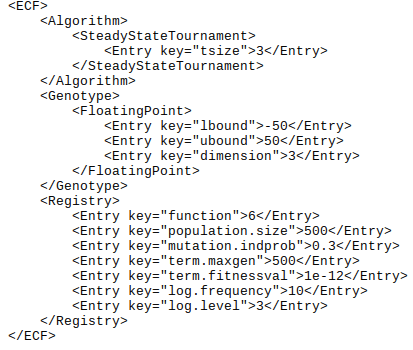
\includegraphics[scale=0.6]{images/xml2}
\caption{Primjer konfiguracijske datoteke}
\end{figure}

\section{Korišteni klasifikatori}



U ovom radu ćemo implementirati dva različita klasifikatora genetskog programiranja. To su :

\begin{itemize}
\item Regresijski GP (klasifikacijski aritmetički izrazi)
\item Regresijski GP uz glasanje - posebno stablo za svaku klasu
\end{itemize}


Regresijski GP s jednim stablom uspoređuje numeričke vrijednosti dobivene evaluacijom stabla s intervalima definiranim za svaku klasu. Razred kojem primjer pripada je onaj u čijem se intervalu nalazi dobivena numerička vrijednost. Funkcijom dobrote potom određujemo uspješnost predviđanja klasa svake jedinke.

Kod regresijskog GP-a uz glasanje svaka klasa ima definirano svoje stablo.  Tijekom evaluacije računamo izlaznu numeričku vrijednost za svako od stabala. Odlučujuće je ono stablo koje daje najmanju apsolutnu vrijednost.
 

Tada u slučaju da imamo tri klase, dakle tri stabla, možemo dobiti sljedeće vrijednost za svako od stabala: \\
stablo A: 3 \\
stablo B: 1.5 \\
stablo C: -2 \\

Recimo da primjer odgovara klasi B. Odlučujuće stablo je stablo B budući da upravo ono ima najmanju apsolutnu vrijednost. Time je jedinka dobro klasificirala zadani primjer.


\section{Funkcije čvorova}

Stabla odluke se sastoje od skupa funkcijskih znakova i skupa završnih znakova. U skup završnih znakova spadaju atributi klasifikacijskog problema. Ako je ukupan broj atributa jednak $n$ varijable tada imaju oznake od $x_0$ do $x_{n-1}$. Prilikom evaluacije, za vrijednosti varijabli iz skupa završnih znakova uzimaju se odgovarajuće vrijednosti iz skupa podataka definiranih za svaki problem klasifikacije.

U skup funkcijskih znakova spadaju:

\begin{itemize}
\item Aritmetički operatori
\item Sinus, kosinus
\item Max, min
\item Sqrt, Log
\item IfPositive
\item IfLessThanEq
\end{itemize}

U nastavku ćemo se pobliže upoznati s njima.

U aritmetičke operatore koje koristimo spadaju zbrajanje (+), oduzimanje (-), množenje (*) i dijeljenje (/). Pored njih, koristit ćemo i funkcije sinusa i kosinusa. 

Ostale korištene funkcije je potrebno implementirati unutar radnog okruženja ECF-a. Pri tome im je potrebno definirati pridružena svojstva \textbf{nArguments\_} koje označava broj djece koje će čvor s navedenom funkcijom imati te \textbf{name\_} koje označava ime navedene funkcije. U svakoj definiranoj funkciji je potrebno implementirati metodu \textbf{execute} u kojoj vrijednosti čvorova djece dohvaćamo pomoću metode \textbf{getNextArgument}. Izlazna vrijednost čvora je vrijednost dobivena primjenom odgovarajuće funkcije na jedno ili više čvorova djece.


\textit{Max} i \textit{Min} funkcije definiraju čvorove koji imaju dvoje djece. \textit{Max} funkcija vraća vrijednost onog djeteta koje ima veću vrijednost, dok \textit{Min} funkcija vraća manju od vrijednosti svoje djece.


Funkcija \textit{Sqrt} definira čvor koji ima jedno dijete te vraća korijen apsolutne vrijednosti tog djeteta.

Kod funkcije \textit{Log} je potrebno pripaziti na vrijednost koju joj predajemo. Budući da je logaritamska funkcija definirana samo za pozitivne vrijednosti veće od nule, u slučaju da je vrijednost djeteta manja ili jednaka nuli funkcija vraća logaritam od jedan, to jest nula.

\textit{IfPositive} definira čvor koji ima troje djece. U slučaju da je vrijednost prvog djeteta veća od 0 vraća vrijednost drugog djeteta, a inače vraća vrijednost trećeg.


\textit{IfLessThanEq} definira čvor koji ima četvero djece. U slučaju da je vrijednost prvog djeteta manja ili jednaka vrijednosti drugog vraća vrijednost trećeg djeteta, a u suprotnom slučaju vrijednost četvrtog djeteta.

Uvođenje logičkih izraza pored onih aritmetičkih je važno jer omogućava veću raznolikost rješenja i pomaže u preciznijoj evoluciji stabala. 

\section{Funkcije dobrote}

Funkcija dobrote koju ćemo koristiti u treniranju klasifikatora je \textit{F1 score}. Nastala je iz matrice (\textit{confusion matrix}) koja omogućava vizualizaciju uspješnosti algoritma, obično nadziranog učenja kod problema umjetne inteligencije među koje spada i problem klasifikacije.

Sastoji se od dvije dimenzije ("stvarno" i "predviđeno") i identičnog skupa klasa u obje dimenzije. 

Za primjer možemo uzeti klasifikator koji razvrstava pse, mačke i zečeve u njihove pripadajuće klase. Ako uzmemo skup od 27 životinja - 8 mačaka, 6 pasa i 13 zečeva, rezultati nakon klasifikacije bi mogli izgledati ovako:

\begin{center}
\begin{tabular}{|c|c|c|c|c|}
\hline
& & \multicolumn{3}{|c|}{Predviđeno} \\
\hline
& & Mačka & Pas & Zec \\
\hline
\multirow{3}{4em}{Stvarno} & Mačka & 5 & 3 & 0 \\

& Pas & 2 & 3 & 1 \\

& Zec & 0 & 2 & 11 \\
\hline

\end{tabular}
\end{center}

Od osam mačaka, klasifikator je za tri predvidio da su psi, a od šest pasa za jednog je predvidio da je zec, a za dva da su mačke. Svi pogoci su prikazani dijagonalom pa je lako vidjeti sve pogreške.

Matrica iz koje ćemo dobiti funkciju dobrote ima dva retka i dva stupca sa sljedećim mogućim vrijednostima za klasu koju analiziramo:

\begin{itemize}
\item \textit{false positive (FP)} - Svrstavanje pogrešnog primjerka u klasu
\item \textit{false negative (FN)} - Primjerci klase koji su svrstani u neku drugu klasu
\item \textit{true positive  (TP)} - Pogodak
\item \textit{true negative  (TN)} - Točno neprihvaćanje primjerka u klasu

\end{itemize}

Za navedeni primjer i klasu Mačka, dobili bi sljedeću matricu.

\begin{center}
\begin{tabular}{|c|c|}
\hline
5 TP (točno svrstane mačke) & 3 FN (mačke svrstane u pse) \\
\hline
2 FP (psi svrstani u mačke) & 17 TN (sve ne-mačke svrstane u druge klase) \\
\hline
\end{tabular}
\end{center}

Naša funkcija dobrote će tada imati oblik:

\[ F1 = \frac{2 * TP}{2 * TP + FP + FN} \]

Moguće vrijednosti su iz intervala $[0, 1]$ gdje veći broj predstavlja veću dobrotu rješenja. Za probleme s više klasa uzima se prosječna vrijednost funkcije dobrote za sve klase.



\section{Parametri i konfiguracijske datoteke}

Parametre zadajemo u konfiguracijskoj datoteci XML formata koju je potrebno predati prilikom inicijaliziranja ECF-a. Tu možemo definirati mehanizme križanja, veličinu populacije, vjerojatnost mutacije, minimalnu i maksimalnu dubinu stabla i druge. 

U slučaju ne navođenja nekog od  parametara, uvode se sljedeće pretpostavljene vrijednosti: 

\begin{itemize}
\item Veličina populacije: 100
\item Vjerojatnost mutacije: 0.3
\item Prekid: 50 generacija bez napretka najbolje jedinke
\end{itemize}

Parametri genotipa koji će nama biti od značaja su \textit{functionset} pomoću kojeg definiramo skup funkcijskih znakova te \textit{terminalset} koji predstavlja skup završnih znakova. Skup završnih znakova ćemo u svim slučajevima definirati oznakama od $x_0$ do $x_{n-1}$ gdje $n$ predstavlja broj atributa problema.

Pored navedenih možemo definirati i parametar \textit{classesNum} koji predstavlja broj klasa koji koristimo u klasificiranju. U slučaju ne navođenja navedenog parametra koristi se pretpostavljena vrijednost dva.

Primjer parametarske datoteke gdje možemo vidjeti navedene atribute nalazi se na slici 4.2.

\begin{figure}[htb]
\centering
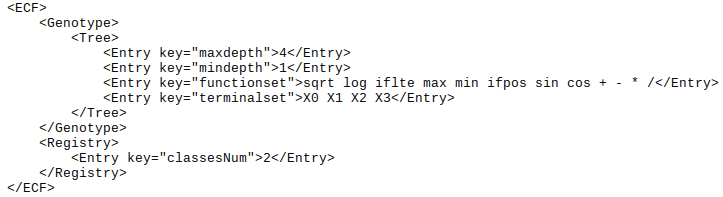
\includegraphics[scale=0.6]{images/xml}
\caption{Primjer konfiguracijske datoteke}
\end{figure}

Kod definiranja intervala klasa koristimo datoteku definiranu parametrom \textit{classesfile}. U slučaju ne navođenja parametra koristi se pretpostavljeni naziv \textit{classes.txt}. Pomoću ove datoteke definiramo sve klase koje koristimo kao i intervale kojima pojedina klasa pripada. Ako datoteka ne postoji, koriste se pretpostavljene klase s oznakama od $0$ do $n-1$ gdje n predstavlja broj klasa definiranih parametrom \textit{classesNum}. Za intervale se koriste negativna i pozitivna potencija broja dva, gdje eksponent intervala odgovara numeričkoj oznaci klase. U klasi $n-1$ definiramo dva intervala koja pokrivaju sve preostale realne vrijednosti.

Naprimjer, ako smo definirali postojanje tri klase bez datoteke sa konfiguracijom dobit ćemo sljedeće vrijednosti intervala:

\begin{itemize}
\item Klasa 0: $[-1,  1]$
\item Klasa 1: $[-2, -1] \cup [1, 2]$
\item Klasa 2: $(-\infty, -2] \cup [2, +\infty)$

\end{itemize}

Primjer strukture datoteke za definiranje razreda nalazi se na slici 4.3.

\begin{figure}[htb]
\centering
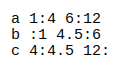
\includegraphics[scale=0.6]{images/klase}
\caption{Primjer definiranja klasa}
\end{figure}

Na početku retka definirano je ime klase, a intervale odvajamo dvotočkama.
Beskonačne vrijednosti označavamo ne navođenjem vrijednosti s odgovarajuće strane intervala.

Za primjer naveden na slici definirane su tri klase i intervali:

\begin{itemize}
\item Klasa a: $[1,4] \cup [6,12]$
\item Klasa b: $(-\infty, 1] \cup [4.5,6]$
\item Klasa c: $[4, 4.5] \cup [12, +\infty)$
\end{itemize}


Primjere za učenje definiramo u datoteci definiranoj parametrom \textit{inputfile} s pretpostavljenom vrijednosti \textit{learning.txt} u kojoj navodimo atribute svakog primjera i razred kojem pripada.

Svaki primjer je napisan u novom retku, a atributi su odvojeni zarezima. Kod primjera s $n$ atributa imat ćemo $n+1$ zapisa u retku gdje posljednji predstavlja klasu.

Na slici 4.4 prikazana je datoteka za učenje čiji primjeri imaju četiri atributa i dva razreda.


\begin{figure}[htb]
\centering
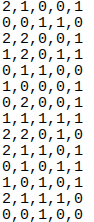
\includegraphics[scale=0.5]{images/learning}
\caption{Datoteka sa primjerima za učenje}
\end{figure}


Datoteka \textit{test.txt} je pretpostavljane vrijednost parametra \textit{testfile} u kojoj se nalaze primjeri za ispitivanje koji imaju identičnu strukturu.

Detaljnije objašnjenje o atributima i šta točno znače za navedene datoteke ćemo opisati u sljedećem poglavlju.

Ime datoteke u koju se zapisuju rezultati određeno je parametrom \textit{resultsfile} koji ima pretpostavljenu vrijednost \textit{results.txt}.

U datoteci se za svaku generaciju zapisuje broj generacije i najveće vrijednosti dobrote skupa za učenje i testiranje. Vrijednosti su odvojene zarezima. Primjer je prikazan na slici 4.5.

\begin{figure}[htb]
\centering
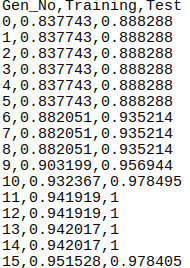
\includegraphics[scale=0.5]{images/rezultati}
\caption{Struktura datoteke sa rezultatima}
\end{figure}



\chapter{Primjena i analiza rezultata}

Implementirane klasifikatore ćemo primijeniti na tri primjera problema klasifikacije. Prvi je vjerojatno najpoznatiji skup podataka za problem klasifikacije u kojem je cilj klasificirati različite porodice cvijeta iris. Drugi problem je problem klasifikacije stakla na osnovu svojstava i kemijskog sastava. Posljednji primjer je problem klasifikacije kvalitete automobila. Svi primjeri će biti testirani sa najviše 50 000 evaluacija.

\section{\textit{Iris flower data set}}

\textit{Iris flower data set} je vjerojatno najpoznatiji skup podataka koji se koristi kod problema klasifikacije. Predstavio ga je Ronald Fisher 1936. godine u svom radu \textit{The use of multiple measurements in taxonomic problems}.

Podaci se sastoje od tri klase po 50 primjeraka gdje je svaki primjerak definiran sa četiri atributa. Klase predstavljaju tri porodice cvijeta iris - porodice su \textit{iris setosa, iris versicolor, iris virginica}.

Atributi koji se koriste su:
\begin{itemize}
\item dužina lapa
\item širina lapa
\item dužina latica
\item širina latica
\end{itemize}

Sve vrijednosti su predstavljene u centimetrima.

Nekoliko uzoraka je prikazano sljedećom tablicom.

\begin{center}
\begin{tabular}{|c|c|c|c|c|c|}
\hline
Dužina lapa & Širina lapa & Dužina latica & Širina latica & Porodica & Oznaka \\
\hline
5.1 & 3.5 & 1.4 & 0.2 & \textit{I. setoosa} & 0 \\
\hline
4.9 & 3.0 & 1.4 & 0.2 & \textit{I. setosa} & 0\\
\hline
7.0 & 3.2 & 4.7 & 1.4 & \textit{I. versicolor} & 1\\
\hline
6.4 & 3.2 & 4.5 & 1.5 & \textit{I. versicolor} & 1\\
\hline
6.3 & 3.3 & 6.0 & 2.5 & \textit{I. virginica} & 2\\
\hline
5.8 & 2.7 & 5.1 & 1.9 & \textit{I. virginica} & 2\\
\hline
\end{tabular}
\end{center}

Primjer će se ispitati na različitim kombinacijama veličine populacije i faktora mutacije. Veličine populacije tijekom testiranja su 50, 100, 200 i 500, a faktori mutacije 0.3, 0.5, 0.7 i 0.9.

U početku ćemo na populaciji veličine 100 jedinki ispitati za koji faktor mutacije postižemo najbolje rezultate, potom će se s tim faktorom ispitati i ostale veličine.

Tijekom učenja klasifikatora ujedno ćemo u svakoj generaciji ispitati i uspješnost klasificiranja na skupu za ispitivanje. U svim rezultatima omjer primjera za učenje i ispitivanje je 70:30.

Faktor mutacije s kojim su postignuti najbolji rezultati je 0.7, kao što je i vidljivo na slici 5.1.

Detaljnija analiza za različite veličine populacije je prikazana na slici 5.2.

\begin{figure}[htb]
\centering
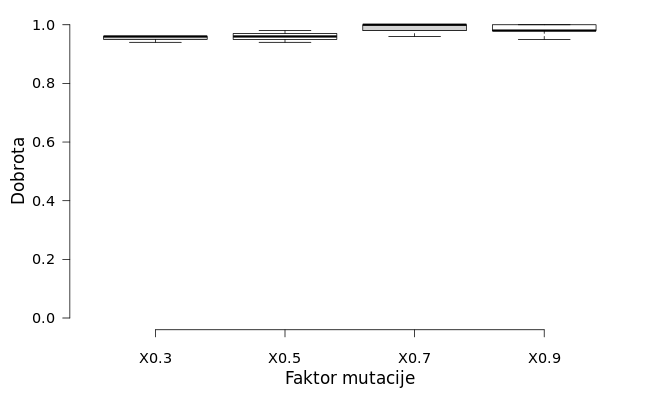
\includegraphics[scale=0.5]{grafovi/boxplotIrisSTest}
\caption{Regresijski GP s jednim stablom populacije veličine 100 ispitan s različitim faktorima mutacije - problem Iris}
\end{figure}

\begin{figure}[htb]
\centering
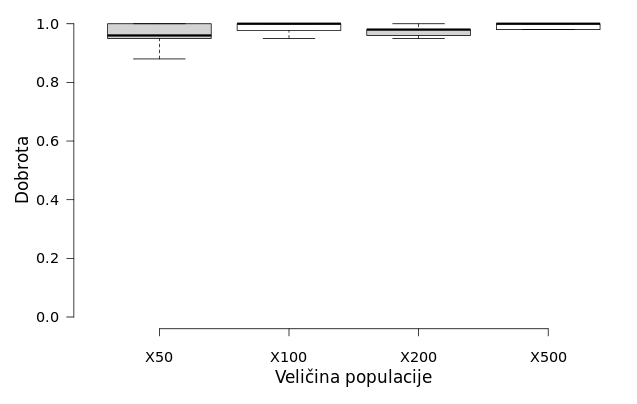
\includegraphics[scale=0.5]{grafovi/boxplotIrisS}
\caption{Regresijski GP s jednim stablom različitih veličina populacije ispitan s faktorom mutacije 0.7 - problem Iris}
\end{figure}


Isti način ispitivanja ćemo primjeniti i na regresijski GP s više stabala.
Na slici 5.3 se uočava da se najbolji rezultati postižu za faktor mutacije 0.7, a rezultati za više populacija su vidljivi na slici 5.4.

\begin{figure}[htb]
\centering
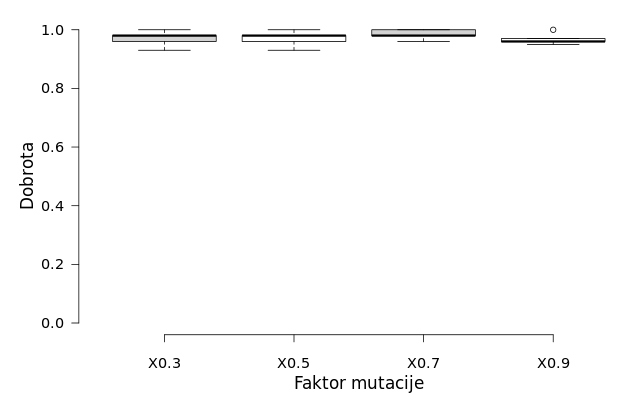
\includegraphics[scale=0.5]{grafovi/boxplotIrisMTest}
\caption{Regresijski GP s više stabala populacije veličine 100 ispitan s različitim faktorima mutacije - problem Iris}
\end{figure}

\begin{figure}[htb]
\centering
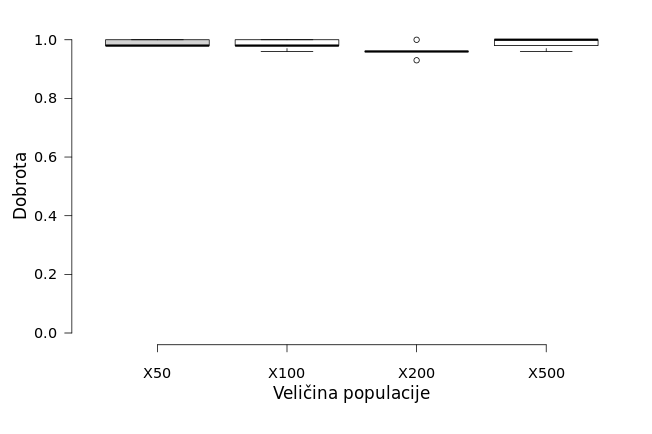
\includegraphics[scale=0.5]{grafovi/boxplotIrisM}
\caption{Regresijski GP s više stabala različitih veličina populacije ispitan s faktorom mutacije 0.7 - problem Iris}
\end{figure}

\begin{figure}[htb]
\centering
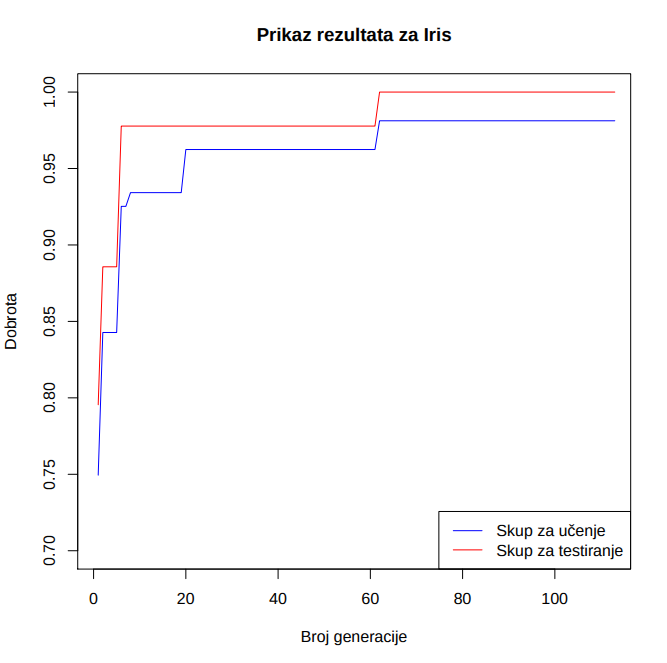
\includegraphics[scale=0.45]{grafovi/iris1}
\caption{Klasifikator s jednim stablom - problem Iris}
\end{figure}


Detaljniji graf rezultata s izraženom dobrotom tijekom svake generacije za veličinu populacije od 100 jedinki i s faktorom mutacije 0.3 primjenom regresijskog GP-a s jednim stablom je prikazan na slici 5.5. Primjer regresijskog GP-a uz više stabala s istim parametrima se nalazi na slici 5.6. Na oba grafa su prikazane najbolje jedinke u svakoj iteraciji.

Možemo zaključiti da klasifikator jako brzo dolazi do zadovoljavajućeg rješenja pomoću kojeg može sa 100\% uspješnosti predvidjeti klasu kojoj pripadaju primjeri za ispitivanje.

Kod regresijskog GP-a s više stabala vidimo da postižemo slične rezultate no da klasifikator uz dosta manje generacija dolazi do zadovoljavajućih rezultata.
 
 
\begin{figure}[htb]
\centering
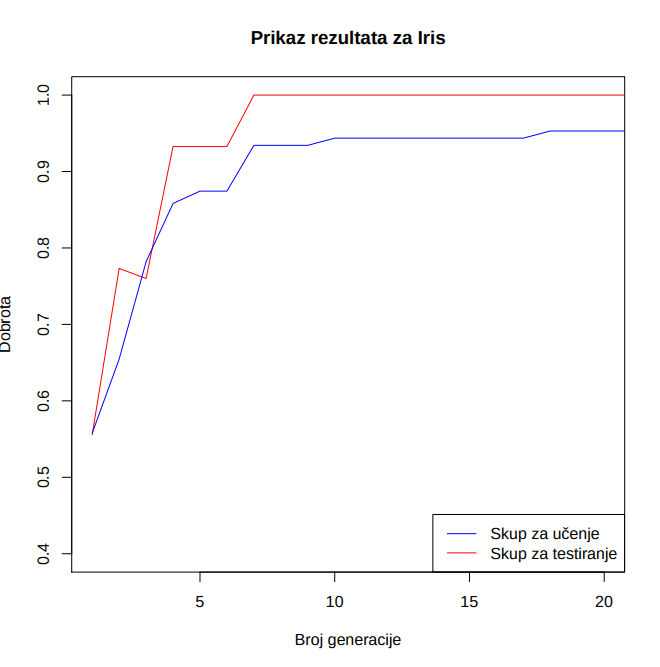
\includegraphics[scale=0.45]{grafovi/iris2}
\caption{Klasifikator s više stabala - problem Iris}
\end{figure}

Budući da se radi o problemu sa samo tri klase i početna populacija postiže rezultate s kojima može klasificirati primjere za ispitivanje s uspješnosti većom od 50\%.

Kako bi detaljnije ispitali uspješnost rada klasifikator, primjeniti ćemo ih i na problem u kojem je cilj raspodijeliti primjere između većeg broja klasa.


\subsection{Klasifikacija stakla}

Sljedeći problem na kojem ćemo testirati klasifikatore je problem identifikacije vrste stakla. Američka agencija \textit{Forensic Science Service} je testirala svojstva i kemijski sastav sedam vrsta stakala.

U svoj analizi testirali su sljedeća svojstva i udjele sastojaka:
\begin{itemize}
\item Lom svjetla
\item Natrij, Magnezij, Aluminij
\item Silicij, Kalij, Kalcij
\item Barij, Željezo

\end{itemize}

Navedeno će ujedno biti atributi kojima ćemo učiti klasifikatore.

Podaci se sastoje od 6 vrste stakla od kojih svi nemaju jednak broj primjera:

\begin{itemize}
\item Obrađeno staklo prozora zgrada - 70 primjeraka
\item Neobrađeno staklo prozora zgrada - 75 primjeraka
\item Obrađeno staklo prozora vozila - 17 primjeraka
\item Staklo posuda - 13 primjeraka
\item Stolno posuđe - 9 primjeraka
\item Staklo automobilskih farova - 29 primjeraka

\end{itemize}

Vidimo da se problem sastoji od većeg broja atributa i klasa, te da su brojevi primjeraka za pojedinu klasu dosta neuravnoteženi zbog čega možemo očekivati da će klasifikatorima biti puno teže pravilno odrediti klase.

Primjer će se testirati na isti način kao i prethodni.

\begin{figure}[htb]
\centering
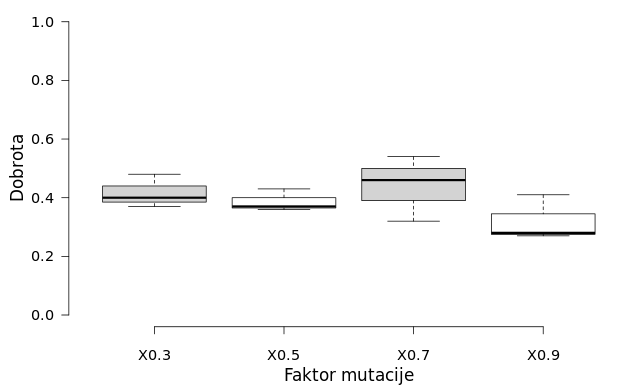
\includegraphics[scale=0.5]{grafovi/boxplotGlassSTest}
\caption{Regresijski GP s jednim stablom populacije veličine 100 ispitan s različitim faktorima mutacije - problem klasifikacije stakla}
\end{figure}

\begin{figure}[htb]
\centering
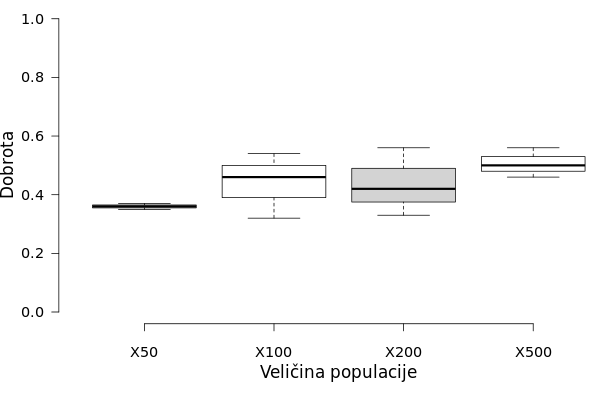
\includegraphics[scale=0.5]{grafovi/boxplotGlassS}
\caption{Regresijski GP s jednim stablom različitih veličina populacije ispitan s faktorom mutacije 0.7 - problem klasifikacije stakla}
\end{figure}

\begin{figure}[htb]
\centering
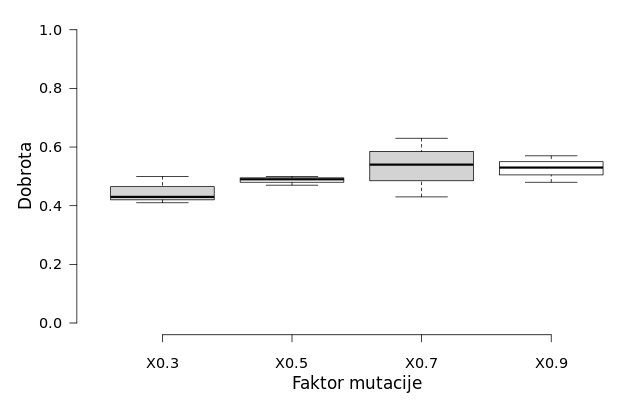
\includegraphics[scale=0.5]{grafovi/boxplotGlassMTest}
\caption{Regresijski GP s više stabala populacije veličine 100 ispitan s različitim faktorima mutacije - problem klasifikacije stakla}
\end{figure}

\begin{figure}[htb]
\centering
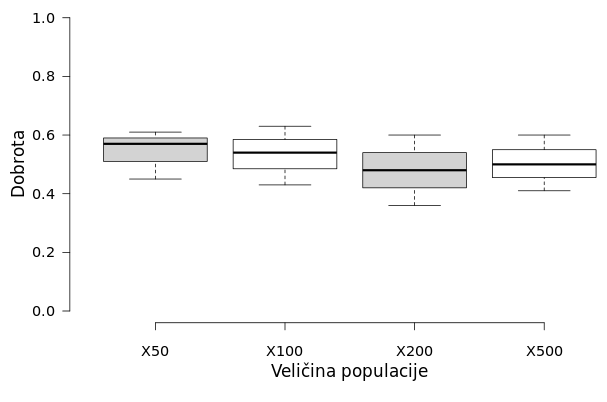
\includegraphics[scale=0.5]{grafovi/boxplotGlassM}
\caption{Regresijski GP s više stabala različitih veličina populacije ispitan s faktorom mutacije 0.7 - problem klasifikacije stakla}
\end{figure}

\begin{figure}[htb]
\centering
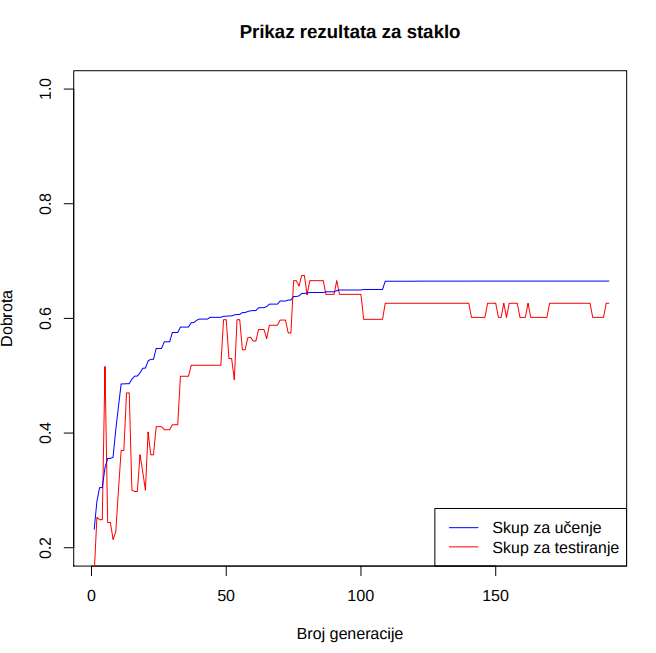
\includegraphics[scale=0.45]{grafovi/staklo1-3}
\caption{Klasifikator s jednim stablom - problem klasifikacije stakla}
\end{figure}


\begin{figure}[htb]
\centering
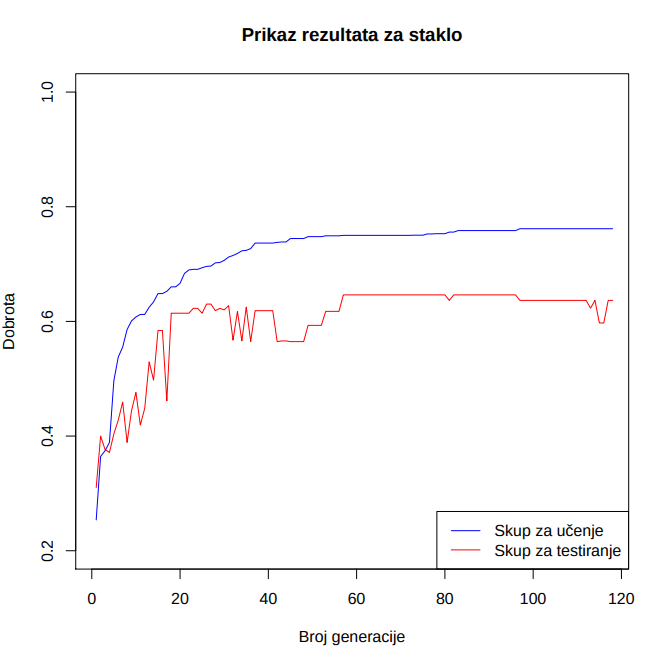
\includegraphics[scale=0.45]{grafovi/staklo2-3}
\caption{Klasifikator s više stabala - problem klasifikacije stakla}
\end{figure}

Na slikama 5.7 i 5.8 se nalaze rezultati testiranja klasifikatora s jednim stablom. Na slikama 5.9 i 5.10 su rezultati za klasifikator s više stabala.

Ponovno možemo primijetiti da klasifikator s više stabala dolazi do sličnih ili boljih rezultata u značajno manjem broju generacija. (Slike 5.11 i 5.12) Veći faktor mutacije obično dovodi i do boljih rezultata skupa za učenje, no vidimo da to obično ne pomaže točnosti klasifikacije primjera za ispitivanje. U ovom problemu klasifikatoru veliki problem predstavlja neuravnotežen broj primjera za pojedine klase zbog čega ne uspijevamo dobiti veliku točnost. Na rezultate može utjecati i izbor primjera koje koristimo za ispitivanje i učenje zbog čega bi bila potrebna detaljna analiza utjecaja svojstava na rezultate.


\subsection{Ispitivanje automobila}

Treći primjer je problem određivanja kvalitete automobila. Automobili se ocjenjuju na temelju sljedećih značajki:

\begin{itemize}
\item Cijena (vrlo visoka, visoka, srednja, niska)
\item Cijena održavanja (vrlo visoka, visoka, srednja, niska)
\item Broj vrata (dva, tri, četiri, pet i više)
\item Broj ljudi (dva, četiri, pet i više)
\item Veličina pretinca za prtljagu (mala, srednja, velika)
\item Sigurnost automobila (mala, srednja, velika)
\end{itemize}

Cilj je automobil svrstati u jednu od četiri klase: neprihvatljiv, prihvatljiv, dobar, vrlo dobar.

Dostupno je 1728 primjeraka za zadani problem koji će se koristiti u omjeru 70:30 za učenje i ispitivanje na isti način kao i u prethodnim primjerima.

Ispitivanjem prikazanim na slici 5.13 je utvrđeno da se najbolji rezultati kod regresijskog GP-a s jednim stablom postižu s faktorom mutacije 0.5. Daljnje ispitivanja za različite veličine populacija prikazano je na slici 5.14.

\begin{figure}[htb]
\centering
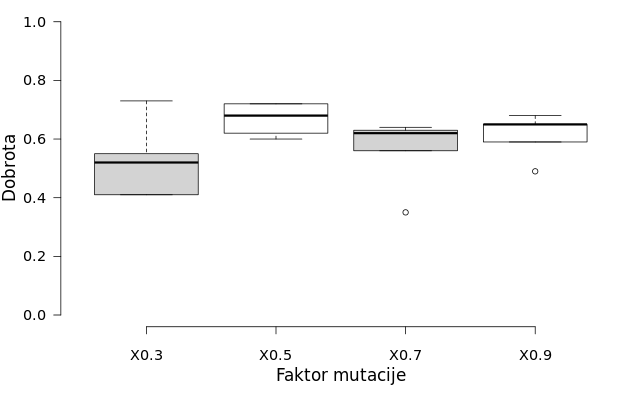
\includegraphics[scale=0.5]{grafovi/boxplotCarSTest}
\caption{Regresijski GP s jednim stablom populacije veličine 100 ispitan s različitim faktorima mutacije - problem ispitivanja automobila}
\end{figure}

\begin{figure}[htb]
\centering
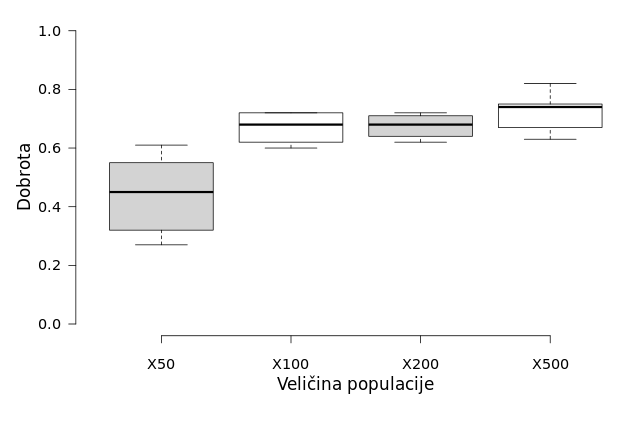
\includegraphics[scale=0.5]{grafovi/boxplotCarS}
\caption{Regresijski GP s jednim stablom različitih veličina populacije ispitan s faktorom mutacije 0.5 - problem ispitivanja automobila}
\end{figure}




Isti postupak ćemo ponoviti i za regresijski GP s više stabala. Na slici 5.16 se nalaze rezultati ispitivanja za različite veličine populacija uz faktor mutacije 0.7 koji je dobiven ispitivanjem prikazanim na slici 5.15.

Prikaz rezultata za svaku generaciju uz veličinu populacije od 100 jedinki i s faktorom mutacije 0.3 nalazi se na slikama 5.17 i 5.18.



Porastom veličine populacije povećava se i kvaliteta rješenja. U ovom slučaju regresijski GP s jednim stablom postiže djelomično bolja rješenja. Potrebno je naglasiti da je klasifikator s jednim stablom puno manje računalno zahtjevan i iako klasifikator s više stabala do rješenja obično dolazi u manjem broju generacija, vrijeme koje je potrebno za izračune je puno duže.

\begin{figure}[htb]
\centering
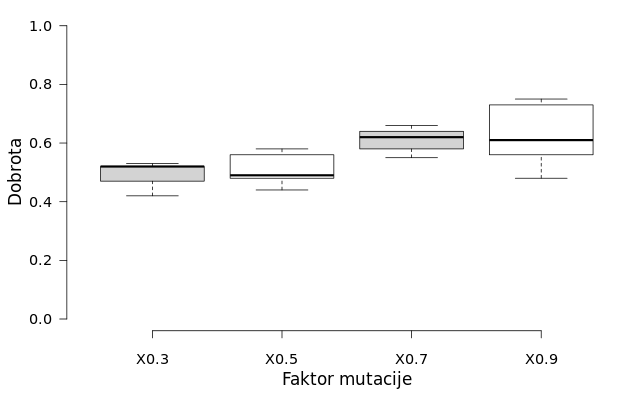
\includegraphics[scale=0.5]{grafovi/boxplotCarMTest}
\caption{Regresijski GP s više stabala populacije veličine 100 ispitan s različitim faktorima mutacije - problem ispitivanja automobila}
\end{figure}

\begin{figure}[htb]
\centering
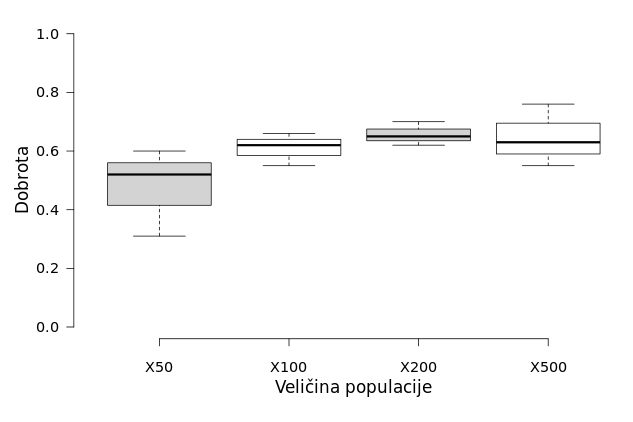
\includegraphics[scale=0.5]{grafovi/boxplotCarM}
\caption{Regresijski GP s više stabala različitih veličina populacije ispitan s faktorom mutacije 0.7 - problem ispitivanja automobila}
\end{figure}

\begin{figure}[htb]
\centering
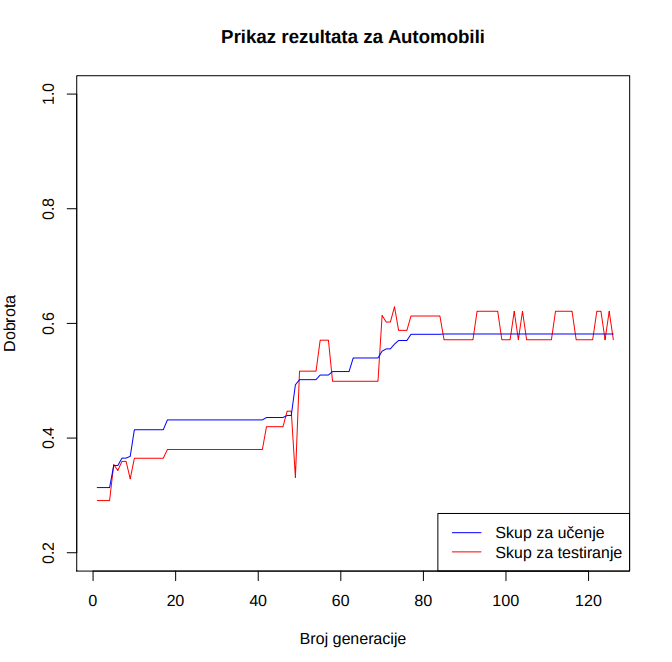
\includegraphics[scale=0.45]{grafovi/automobili1-3}
\caption{Klasifikator s jednim stablom - problem ispitivanja automobila}
\end{figure}


\begin{figure}[htb]
\centering
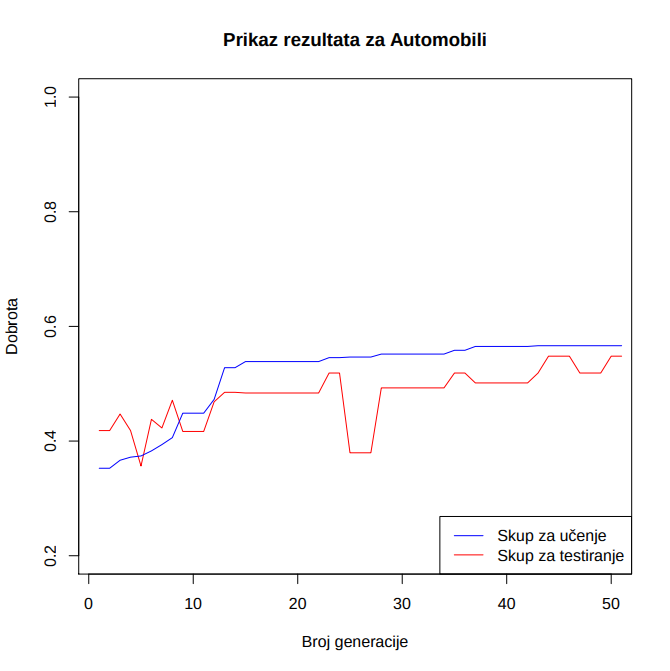
\includegraphics[scale=0.45]{grafovi/automobili2-3}
\caption{Klasifikator s više stabala - problem ispitivanja automobila}
\end{figure}


\chapter{Zaključak}
U radu smo opisali genetsko programiranje i problem klasifikacije te se malo pobliže upoznali sa načinom na koji rade. Vidjeli smo da se genetsko programiranje može uspješno koristiti za učenje klasifikatora no da je potrebno pripaziti na moguće probleme poput pojavljivanja pretjerane složenosti i prevelikog broja čvorova u stablima. Problemi s više atributa i klasa zahtijevaju i veće računalne resurse zbog čega ponekad nisu najbolje rješenje za velike izračune bez pristupa jačim uređajima. Navedeni klasifikatori se mogu dodatno poboljšati primjenom različitih operatora križanja mutiranja kao i funkcija koje se koriste u čvorovima za izračune. Moguće je i uvođenje skupa podataka kojim bi osigurali da ne dođe do prilagođavanja klasifikatora specifičnim podacima i šumu.



\bibliographystyle{fer}
\bibliography{literatura}
\begin{enumerate}
	\item Riccardo Poli, William B. Langdan, Nicholas F. McPhee, A Field Guide to Genetic Programming. \\
	\emph{http://www.cs.ucl.ac.uk/staff/wlangdon/ftp/papers/poli08\_fieldguide.pdf}

	\item Mehryar Mohri, Afshin Rostamizadeh, Ameet Talwalkar, Foundations of Machine Learning. \\
	\emph{http://www.cs.nyu.edu/~mohri/mlbook/}

	\item Wei-Yin Loh, Classification and regression trees. \\
	\emph{http://www.stat.wisc.edu/~loh/treeprogs/guide/wires11.pdf}
\end{enumerate}


\begin{sazetak}
Problemi klasifikacije su danas jedni od najraširenijih problema s kojima se susrećemo. U radu se opisuje uporaba genetskog programiranja na problem klasifikacije te implementacija i primjena klasifikatora s jednim ili više stabala odluke. Napravljena je analiza njihovog rada te su opisani problemi i moguća poboljšanja.

\kljucnerijeci{ECF, genetsko programiranje, klasifikacija, stabla odluke}
\end{sazetak}

% TODO: Navedite naslov na engleskom jeziku.
\engtitle{Classification of data with genetic programming}
\begin{abstract}
Classification problems are one of the widely spread problems that are encountered in everyday life. Our goal in this thesis is to describe use of genetic programming on classification and implementation of the classifiers with one or more regression trees together with detailed analysis and explanation of possible problems and improvements.

\keywords{ECF, genetic programming, classification, decision trees}
\end{abstract}

\end{document}
